\chapter{Cr�ation d'un nouveau Display}

Ref : TV310315\_TU\_SM \hfill R�dacteur : Serge  Morvan \\


\section{Architecture}
\subsection{Principes}
Un {\tt Display} est un composant, au sens de C$^3$, il peut ainsi b�n�ficier des services du 
composant {\tt GuiAgent} par exemple. L'application n'a aucun lien cod� avec lui. Le design du nouveau compo\-sant 
est compl�tement s�par� du code.
Chaque �l�ment variable poss�de un id. Le contr�leur, instanci� par le {\tt Display} lors de l'initialisation
charge le fichier {\tt .fxml}. On retrouve dans le code du contr�leur les id de la partie graphique.
Pr�conisations : le composant graphique principal est un {\tt Group}, son id est : {\tt view}, chaque {\tt Display}
poss�de un bouton de fermeture, dont l'id est {\tt quit}. Le contr�leur h�rite de la classe {\tt Widget2D} qui offre 
les services de l'interactivit�.
 L'attribut {\tt KEY\_NAME}, ici : {\tt "InstrumentTemplate"} permet au Dock de le rechercher et de l'afficher, lorsque l'item
 associ� est s�lectionn�. Comme ci dessous dans la classe {\tt DockManagerImpl} du module {\tt navisu-app}, lors de
 la cr�ation du Dock :
 {\small 
\begin{verbatim}
instrumentsRadialMenu = RadialMenuBuilder.create()
.centralImage("instrumentsradialmenu150.png")
.createNode(0, "navigation.png",1,"ais.png",1,"template.png",(e)->open("InstrumentTemplate"))
.build();
\end{verbatim}
}
Le nouveau {\tt Display} devra s'enregistrer aupr�s du {\tt IntrumentDriverManagerServices}, dans la classe {\tt AppMain} du module {\tt navisu-launcher}.
{\small
\begin{verbatim}
 // deploy components
 LOGGER.info("\n"
 + componentManager.startApplication(DpAgentImpl.class,
 .....
  InstrumentTemplateImpl.class
  )
  );
  ......
  InstrumentTemplateServices instrumentTemplateServices 
                   = componentManager.getComponentService(InstrumentTemplateServices.class); 
  ......
  instrumentDriverManagerServices.registerNewDriver(instrumentTemplateServices.getDriver());
\end{verbatim}
}
\subsection{Diagramme UML}
La figure ci dessous pr�sente un diagramme simplifi� pour un {\tt Display} appel� {\tt InstrumentTemplate},
%%%%%%%%%%%%%%%%%%%%%%%%%%%%%%%%%%%%%%%%%%%%%%%%%%%%%%%%%%%%%%%%%%%%%%%
\begin{center}
	\framebox[1\width]{
		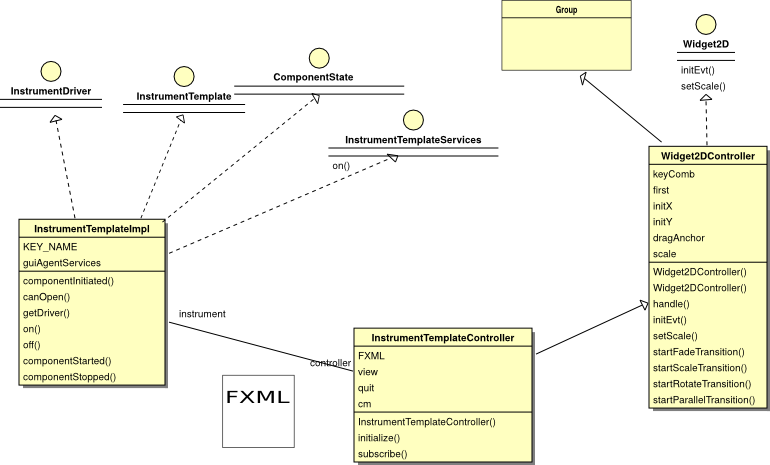
\includegraphics[width=16cm]{images/display/InstrumentTemplate.png}
	}
	\begin{figure}[ht]
		\caption{\label{0}\textit{Diagramme UML simplifi� d'un Display}}
	\end{figure}
\end{center}
%%%%%%%%%%%%%%%%%%%%%%%%%%%%%%%%%%%%%%%%%%%%%%%%%%%%%%%%%%%%%%%%%%%%%%%
\section{Cr�er un nouveau {\tt Display} : {\tt Compass}}
Reprendre le code du {\tt InstrumentTemplate}, �crire les interfaces {\tt Compass} et {\tt CompassServices}, impl�menter
les classes {\tt CompassImpl} et {\tt CompassControler}.Cr�er le fichier graphique {\tt compass.fxml}. Identifier par un id chaque variable.
Reprendre ces variables en mode public dans le contr�leur. Eventuellement ajouter des services, par d�faut
un {\tt Display} offre le service {\tt on()}. Impl�menter les contr�les.
